\begin{enumerate}[label=\thesection.\arabic*,ref=\thesection.\theenumi]
\numberwithin{equation}{enumi}
\numberwithin{figure}{enumi}
\numberwithin{table}{enumi}

\item $AD$ is a diameter of a circle and $AB$ is a chord. If $AD = 34 cm$, $AB = 30 cm$, the distance of $AB$ from the centre of the circle is:
\begin{enumerate}
\item 17cm
\item 15cm
\item 4cm
\item 8cm
\end{enumerate}
\item In Fig. \ref{fig:exemplar/9.10.1/10.3}, if $OA = 5cm, AB = 8cm$ and $OD$ is perpendicular to $AB$, then $CD$ is equal to:
\begin{figure}[H]
\centering
\includegraphics[width=\columnwidth]{exemplar/9.10.1/figs/10.3.jpg}
\caption{}
\label{fig:exemplar/9.10.1/10.3}
\end{figure}
\begin{enumerate}
\item 2cm
\item 3cm
\item 4cm
\item 5cm
\end{enumerate}
\item If $AB = 12 cm, BC = 16 cm$ and $AB$ is perpendicular to $BC$, then the radius of the circle passing through the points $\vec{A},\vec{B}$ and $\vec{C}$ is:
\begin{enumerate}
\item 6cm
\item 8cm
\item 10cm
\item 12cm
\end{enumerate}
\item In Fig. \ref{fig:exemplar/9.10.1/10.4}, if $\angle ABC = 20\degree$ , then $\angle AOC$ is equal to: 
\begin{figure}[H]
\centering
\includegraphics[width=\columnwidth]{exemplar/9.10.1/figs/10.4.jpg}
\caption{}
\label{fig:exemplar/9.10.1/10.4}
\end{figure}
\begin{enumerate}
\item $20\degree$
\item $40\degree$
\item $60\degree$
\item $10\degree$
\end{enumerate}
\item In Fig. \ref{fig:exemplar/9.10.1/10.5}, if $AOB$ is a diameter of the circle and $AC = BC$,then $\angle CAB$ is equal to:
\begin{figure}[H]
\centering
\includegraphics[width=\columnwidth]{exemplar/9.10.1/figs/10.5.jpg}
\caption{}
\label{fig:exemplar/9.10.1/10.5}
\end{figure}
\begin{enumerate}
\item $30\degree$
\item $60\degree$
\item $90\degree$
\item $45\degree$
\end{enumerate}
\item In Fig. \ref{fig:exemplar/9.10.1/10.6}, if $\angle OAB = 40\degree$ , then $\angle ACB$ is equal to:  
\begin{figure}[H]
\centering
\includegraphics[width=\columnwidth]{exemplar/9.10.1/figs/10.6.jpg}
\caption{}
\label{fig:exemplar/9.10.1/10.6}
\end{figure}
\begin{enumerate}
\item $50\degree$
\item $40\degree$
\item $60\degree$
\item $70\degree$
\end{enumerate}
\item In Fig. \ref{fig:exemplar/9.10.1/10.7}, if $\angle DAB = 60\degree , \angle ABD = 50\degree$ , then $\angle ACB$ is equal to:
\begin{figure}[H]
\centering
\includegraphics[width=\columnwidth]{exemplar/9.10.1/figs/10.7.jpg}
\caption{}
\label{fig:exemplar/9.10.1/10.7}
\end{figure}
\begin{enumerate}
\item $60\degree$
\item $50\degree$
\item $70\degree$
\item $80\degree$
\end{enumerate}
\item $ABCD$ is a cyclic quadrilateral such that $AB$ is a diameter of the circle circumscribing it and $\angle ADC = 140\degree$ , then $\angle BAC$ is equal to:
\begin{enumerate}
\item $80\degree$
\item $50\degree$
\item $40\degree$
\item $30\degree$
\end{enumerate}
\item In Fig. \ref{fig:exemplar/9.10.1/10.8}, $BC$ is a diameter of the circle and $\angle BAO = 60\degree$. Then $\angle ADC$ is equal to:
\begin{figure}[H]
\centering
\includegraphics[width=\columnwidth]{exemplar/9.10.1/figs/10.8.jpg}
\caption{}
\label{fig:exemplar/9.10.1/10.8}
\end{figure}
\begin{enumerate}
\item $30\degree$
\item $45\degree$
\item $60\degree$
\item $120\degree$
\end{enumerate}
\item In Fig. \ref{fig:exemplar/9.10.1/10.9}, $\angle AOB = 90\degree$ and $\angle ABC = 30\degree$ , then $\angle CAO$ is equal to:            
\begin{figure}[H]
\centering
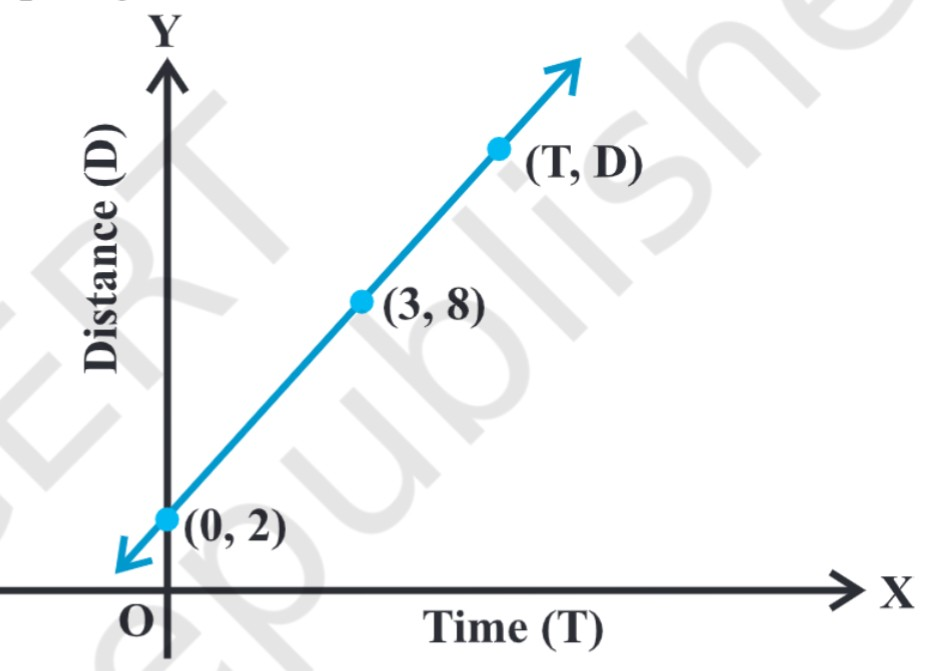
\includegraphics[width=\columnwidth]{exemplar/9.10.1/figs/10.9.jpg}
\caption{}
\label{fig:exemplar/9.10.1/10.9}
\end{figure}
\begin{enumerate}
\item $30\degree$
\item $45\degree$
\item $90\degree$
\item $60\degree$
\end{enumerate}
\item Two chords $AB$ and $CD$ of a circle are each at distances $4 cm$ from the centre The $AB=CD$.
\item Two chords $AB$ and $AC$ of a circle with centre $O$ are an the opposite sides of $OA$ Then $\angle 0AB = \angle 0AC$
\item Two congruent circles with centres 0 and 0 intersect at two points $A$ and $B$ Then $\angle AOB= \angle AOB$
\item Through three collinear points a circle can be drawn
\item A circle of radius $3 cm$ can be drawn through two points $A,B$ such that $AB= 6cm$
\item If AOB is a diameter of a circle and $C$ is a point on the circle, then $AC^2+B^2=AB^2.$
\item $ABCD$ is a cyclic quadrilateral such that $\angle A=90\degree ,\angle B=70\degree, \angle C=95\degree \text{ and }\angle D=105\degree$
\item If A,B,C,D are four points such that $\angle BAC=30\degree, \angle BDC=60\degree$, then D is the centre of the circle through A,B  and C.
\item If A,B,C and D are four points such that $\angle BAC =45\degree \text{ and }\angle BDC=45\degree$, then A,B,C,D are concyclic.
\item In fig \ref{fig:exemplar/9.10.2/1} if AOB is a diameter and $\angle ADC=120\degree \text{ then }\angle CAB=30\degree$
\begin{figure}[h!]
 \begin{center} 
	 \includegraphics[width=\columnwidth]{exemplar/9.10.2/figs/image.jpg}
 \end{center}
\caption{}
	\label{fig:exemplar/9.10.2/1}
\end{figure}
\item If two equal chords of a circle intersect prove that the parts of one chord are separately equal to the parts of the other chord.
\item If non-parallel sides of a trapezium are equal. Prove that it is cyclic
\item If $\vec{P},\vec{Q}$ and $\vec{R}$ are the mid-points of the sides $BC$, $CA$ and $AB$ of a triangle and $AD$ is the perpendicular from $\vec{A}$ on $BC$. Prove that $\vec{P},\vec{Q},\vec{R}$ and $\vec{D}$ are concyclic.
\item $ABCD$ is a parallelogram. A circle through $\vec{A}$, $\vec{B}$ is so drawn that it intersects $AD$ at $\vec{P}$ and $BC$ at $\vec{Q}$. Prove that $\vec{P}$, $\vec{Q}$, $\vec{R}$ and $\vec{D}$ are concyclic.
\item Prove that angle bisector of any angle of a triangle and perpendicular bisector of the opposite side if intersect, they will intersent on the circumcircle of the triangle.
\item If two chords $AB$ and $CD$ of a circle AYDZBWCX intersect at right angles see Fig.\ref{fig:exemplar/9.10.4/1}. Prove that
	\begin{align}
		arc\brak{CXA}+arc\brak{DZB}&=arc\brak{AYD}+arc\brak{AYD}+arc\brak{BWC}\\&=semi-circle
	\end{align}
\begin{figure}[h!]                                   \includegraphics[width=\columnwidth]{exemplar/9.10.4/figs/image1.jpg}                            \caption{}                                       \label{fig:exemplar/9.10.4/1}                    \end{figure}
	\item If $ABC$ is an equilateral triangle inscribed in a circle and $\vec{P}$ be any point on the minor arc $BC$ which does not coincide with $\vec{B}$ or $\vec{C}$. Prove that $PA$ is angle bisector of $\angle BPC$.
	\item In Fig.\ref{fig:exemplar/9.10.4/2}, $AB$ and $CD$ are two chords of a circle intersecting each other at point $\vec{E}$. Prove that 
		\begin{align}
\angle AEC=\frac{1}{2} (\text{Angle subtended by arc CXA at centre}\\ + \text{angle subtended by arc DYB at the centre}).
		\end{align}
	\begin{figure}[h!]                                   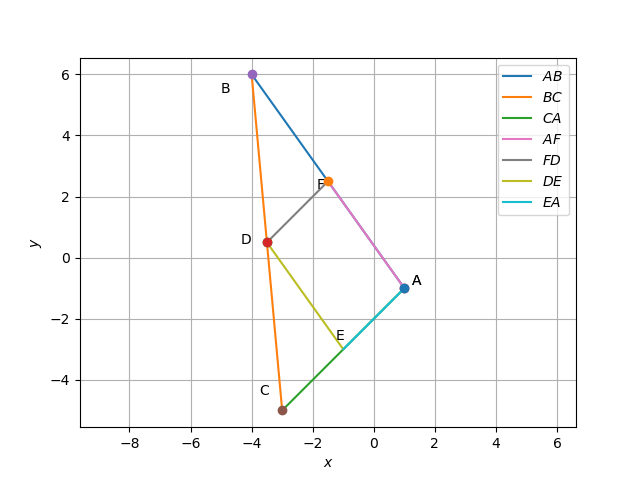
\includegraphics[width=\columnwidth]{exemplar/9.10.4/figs/image2.jpg}                           \caption{}                                       \label{fig:exemplar/9.10.4/2}                    \end{figure}
	\item If bisectors of opposite angles of a cyclic quadrilateral $ABCD$ intersect the circle, circumscribing it at the points $\vec{P}$ and $\vec{Q}$. Prove that $PQ$ is a diameter of the circle.
\item A circle has radius $\sqrt{442}$ cm it is divided into two segments by a chord of length 2cm. Prove that the angle subtended by the chord at a point in major segment is $45\degree$.
\item Two equal chords $AB$ and $CD$ of a circle when produced intersect at a point $\vec{P}$. Prove that $PB=PD$
\item $AB$ and $AC$ are two chords of a circle of radius r such that $AB=2AC$. If $\vec{P}$ and $\vec{Q}$ are the distances of $AB$ and $AC$ from the centre. Prove that $4q^2=p^2+3r^2$.
\item In Fig.\ref{fig:exemplar/9.10.4/3}, $\vec{O}$ is the centre of the circle, $\angle BCO=30\degree$. Find $x$ and $y$.
	\begin{figure}[h!]                                   \includegraphics[width=\columnwidth]{exemplar/9.10.4/figs/image3.jpg}                            \caption{}                                       \label{fig:exemplar/9.10.4/3}                    \end{figure}
	\item In Fig.\ref{fig:exemplar/9.10.4/4}, $\vec{O}$ is the centre of the circle, $BD=OD$ and $CD \bot AB$. Find $\angle CAB$.
		\begin{figure}[h!]                      \includegraphics[width=\columnwidth]{exemplar/9.10.4/figs/image4.jpg}                              \caption{}                                       \label{fig:exemplar/9.10.4/4}                    \end{figure}
\end{enumerate}
